% To generate a PDF from this document, run the following code in R:
%
%   Sweave("algorithms.Rnw")
%   tools::texi2pdf("algorithms.tex")
%
%
\documentclass[final]{siamart171218}
%\VignetteIndexEntry{Algorithms for NMF and topic modeling}
%\VignettePackage{fastTopics}
\usepackage{Sweave}
\usepackage{amsmath}
\usepackage{amssymb}
\usepackage{bm}
\setlength{\oddsidemargin}{0.65in}
\setlength{\evensidemargin}{0.65in}

\title{Algorithms for fitting topic models and non-negative matrix 
  factorizations to count data}
\author{Peter Carbonetto and Matthew Stephens\thanks{Department of 
  Human Genetics and the Research Computing Center, University of 
  Chicago, Chicago, IL}}

\begin{document}

\maketitle

\section{Overview}

This document details the development of efficient algorithms for
minimizing 
\begin{equation}
\ell(L,F) = \ldots
\label{eq:loss}
\end{equation}
subject to all entries of the matrices $F$ and $L$ being
non-negative. (In the discussion and derivations below, we assume $k
\geq 2$---the special case of $k = 1$ is treated in Appendix X.)

Note that we can only obtain a local minium.

This optimization problem can be arrived at in several different
ways. Perhaps the most straightforward and intuitive way is to start
with a basic Poisson model of the count data, in which each Poisson
rate $\lambda_{ij}$ is obtained as a simple linear combination:
\begin{align*}
x_{ij}       &\sim \mathrm{Poisson}(\lambda_{ij}) \\
\lambda_{ij} &=
\label{eq:pnmf}
\end{align*}
where $\mathrm{Poisson}(\lambda)$ denotes the Poisson distribution with
mean $\lambda$. In matrix notation, this gives $\Lambda = LF^T$, which
makes clear that we are representing the Poisson rates as a
non-negative matrix factorization. The loss function to be minimized
\eqref{eq:loss} is precisely the negative log-likelihood of the
Poisson model (with terms that do not depend on either $F$ or $L$
omitted from this expression), so solving \eqref{eq:loss} is
equivalent to computing maximum-likelihood estimates (MLE) of $F$ and
$L$ in model \eqref{eq:pnmf} . Hence, it is now common to refer to
this as ``Poisson non-negative matrix
factorization.''\footnote{Mention the alternative derivation as a
  generalized divergence.}

In addition to gaining mathematical insights into this problem, we
also look closely at the computational aspects, and use these
investigations to help us design efficient algorithms for
solving \eqref{eq:loss}.

\section{Connection to topic modeling}

By optimizing \eqref{eq:loss} subject to the non-negativity
constraints, we are also optimizing a topic model [refs]. Here we make
this connection clear.

{\em Give R code here implementing this transformation.}

\section{An EM algorithm}

{\em Text goes here.}

\section{A stopping criterion}

{\em Text goes here.}

\section{EM, revisited}

{\em Text goes here.}

In this example we embed parts of the examples from the
\texttt{kruskal.test} help page into a \LaTeX{} document:
\begin{Schunk}
\begin{Sinput}
> data(airquality, package = "datasets")
> library("stats")
> kruskal.test(Ozone ~ Month,data = airquality)
\end{Sinput}
\begin{Soutput}
	Kruskal-Wallis rank sum test

data:  Ozone by Month
Kruskal-Wallis chi-squared = 29, df = 4, p-value = 7e-06
\end{Soutput}
\end{Schunk}

which shows that the location parameter of the Ozone distribution
varies significantly from month to month. Finally, we include a
boxplot of the data, using
\begin{Schunk}
\begin{Sinput}
> boxplot(Ozone ~ Month, data = airquality)
\end{Sinput}
\end{Schunk}
\begin{center} 
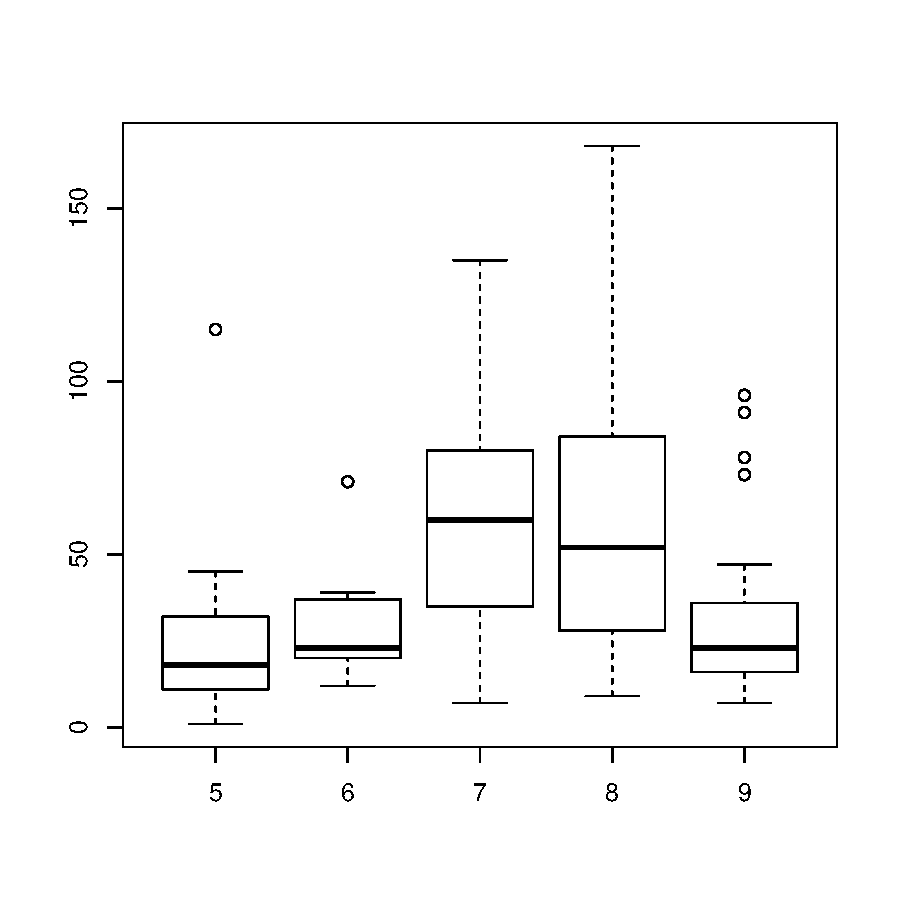
\includegraphics{algorithms-003}
\end{center}

Here is a citation: \cite{lee-2001}.

\appendix

\section{The special case of $k = 1$}

{\em Text goes here.}

\bibliographystyle{siamplain}
\bibliography{algorithms}

\end{document}
